
\subsection{Time references, intervals and CPG sequence}
\label{subsec:intervals}
The variability study addressed in this chapter is based on the characterization of cycle-by-cycle intervals in the rhythm produced by the model CPG.
In our analysis of variability, we assess the presence of linear relationships between the intervals that build the sequence and the cycle-by-cycle period to characterize and unveil similar dynamical invariants as those found in the stomatogastric CPG \parencite{elices_robust_2019}. 
The intervals here analyzed can be measured for any two or three neurons following a robust triphasic rhythm. In the feeding CPG, N1, N2 and N3 represent the three phases, represented in the model by interneurons N1M, N2v and N3t, respectively and in the experimental data by different combinations of moto- and interneurons (see Sec. \ref{subsec:methods experimental intervals}).

\begin{figure}[hbt!]
	\centering
	\begin{minipage}{\textwidth}
		\centering
		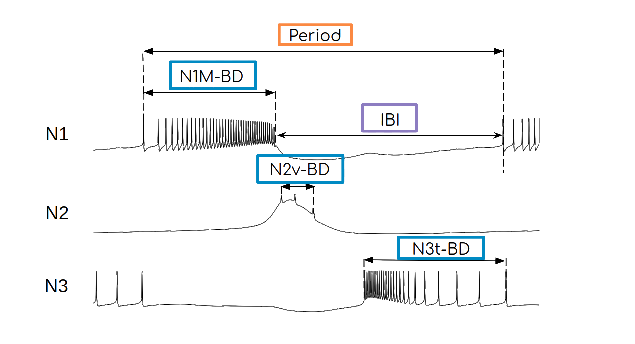
\includegraphics[width=0.8\textwidth]{img/methods-paper-modelo/figure4a.eps} 
		\label{fig:intervals_bd}
	\end{minipage}
	% \hfill
	
	\vspace{1cm}
	\begin{minipage}[t]{\textwidth}
		\centering
		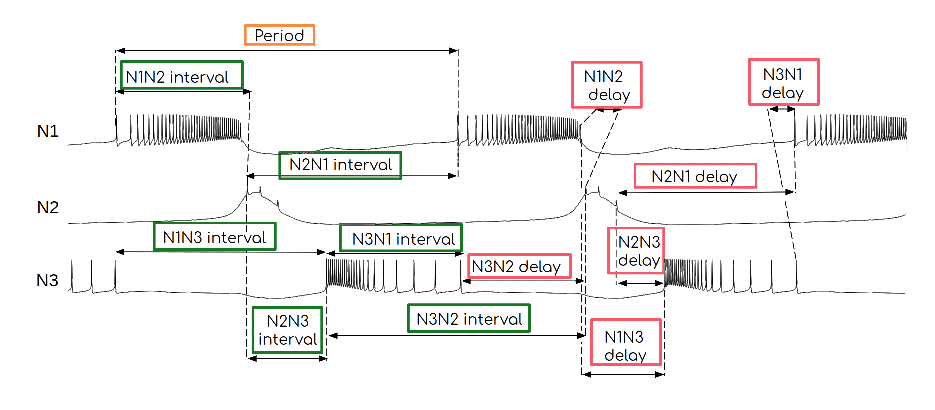
\includegraphics[width=\textwidth]{img/methods-paper-modelo/figure4b.eps} 
		\label{fig:intervals_der}
	\end{minipage}
	
	\caption{\textbf{Panel A}. Individual neuron sequence interval definitions. Each BD label represents the burst duration, defined as the time interval from the first spike to the last spike in the neuron's burst. Period was measured as the interval from the first spike of N1 burst to the first spike of the next N1 burst, covering three phases %(N1M,N2v, N3t) 
		in relation to the activity of the other neurons. IBI represents the interburst interval, defined as the time from the last spike of a neuron's burst to the first one of the next burst in the same neuron.
		\textbf{Panel B}. Definition of intervals involving pairs of neurons. NXNY interval represents interval from NX start to NY start. NXNY delay represents interval from NX end to NY start. Period was measured from N1 start to N1 start, covering the three phases of the CPG rhythm.
	}
	
	\label{fig:intervals}
\end{figure}


Figure \ref{fig:intervals} shows the intervals described from single neuron intervals and intervals defined between two neurons. The definition of each interval is as follows:
\begin{enumerate}
	\item \textbf{Burst Duration (BD)}, measured as the time interval between the first and the last spike of the burst (start to end in the trace of a given neuron).
	\item \textbf{Inter Burst Interval (IBI)}, characterized as the difference between the last spike of a burst and the first one of the next one (end to start in the trace of a given neuron).
	\item \textbf{Period}, which covers the bursts from the three neurons and correspond to a cycle. It is measured as the distance between the first spike of one burst in a neuron and the first spike of the next one on that neuron (start to start).
	\item \textbf{NeuronX-NeuronY interval}, this interval is measured from the start of the burst of neuron X to the start of the burst of neuron Y (start X to start Y).
	\item \textbf{NeuronX-NeuronY delay}, being the time lapse between the burst end of a neuron X and the burst beginning of neuron Y. (end X to start Y).
\end{enumerate}

Note that it is also possible to define those intervals only with the references from two neurons. For example, the intervals conformed based on N1 and N3 intervals would be: N1N3 and N3N1 intervals and N1N3 and N3N1 delay. The intervals corresponding to the third neuron are enclosed in the others defined, e.g., in this example N2 burst and N2N1 delay would be contained in N1N3 delay. This consideration allows the characterization of the variability cycle-by-cycle in cases where it is not possible to define time references for the three neurons in the circuit. 

\subsection{Inducing variability in the model by current injection}
\label{subsec:inj protocol}
The spiking-bursting activity of the model CPG neurons can be modulated by using an additional current injection on each cell, implemented in the \(i_{inj}\) term of equation (\ref{eq:soma}). Depending on the current value applied, the corresponding neuron dynamics changes. While for N2v a change in this injection corresponds to a change in burst frequency (i.e. the number of bursts increases/decreases), for the rest of the neurons in the model a change in \(i_{inj}\) affects burst duration for N3t and SO, and the length of the depolarization phase in N1M.


\begin{figure}[hbt!]
	\centering
	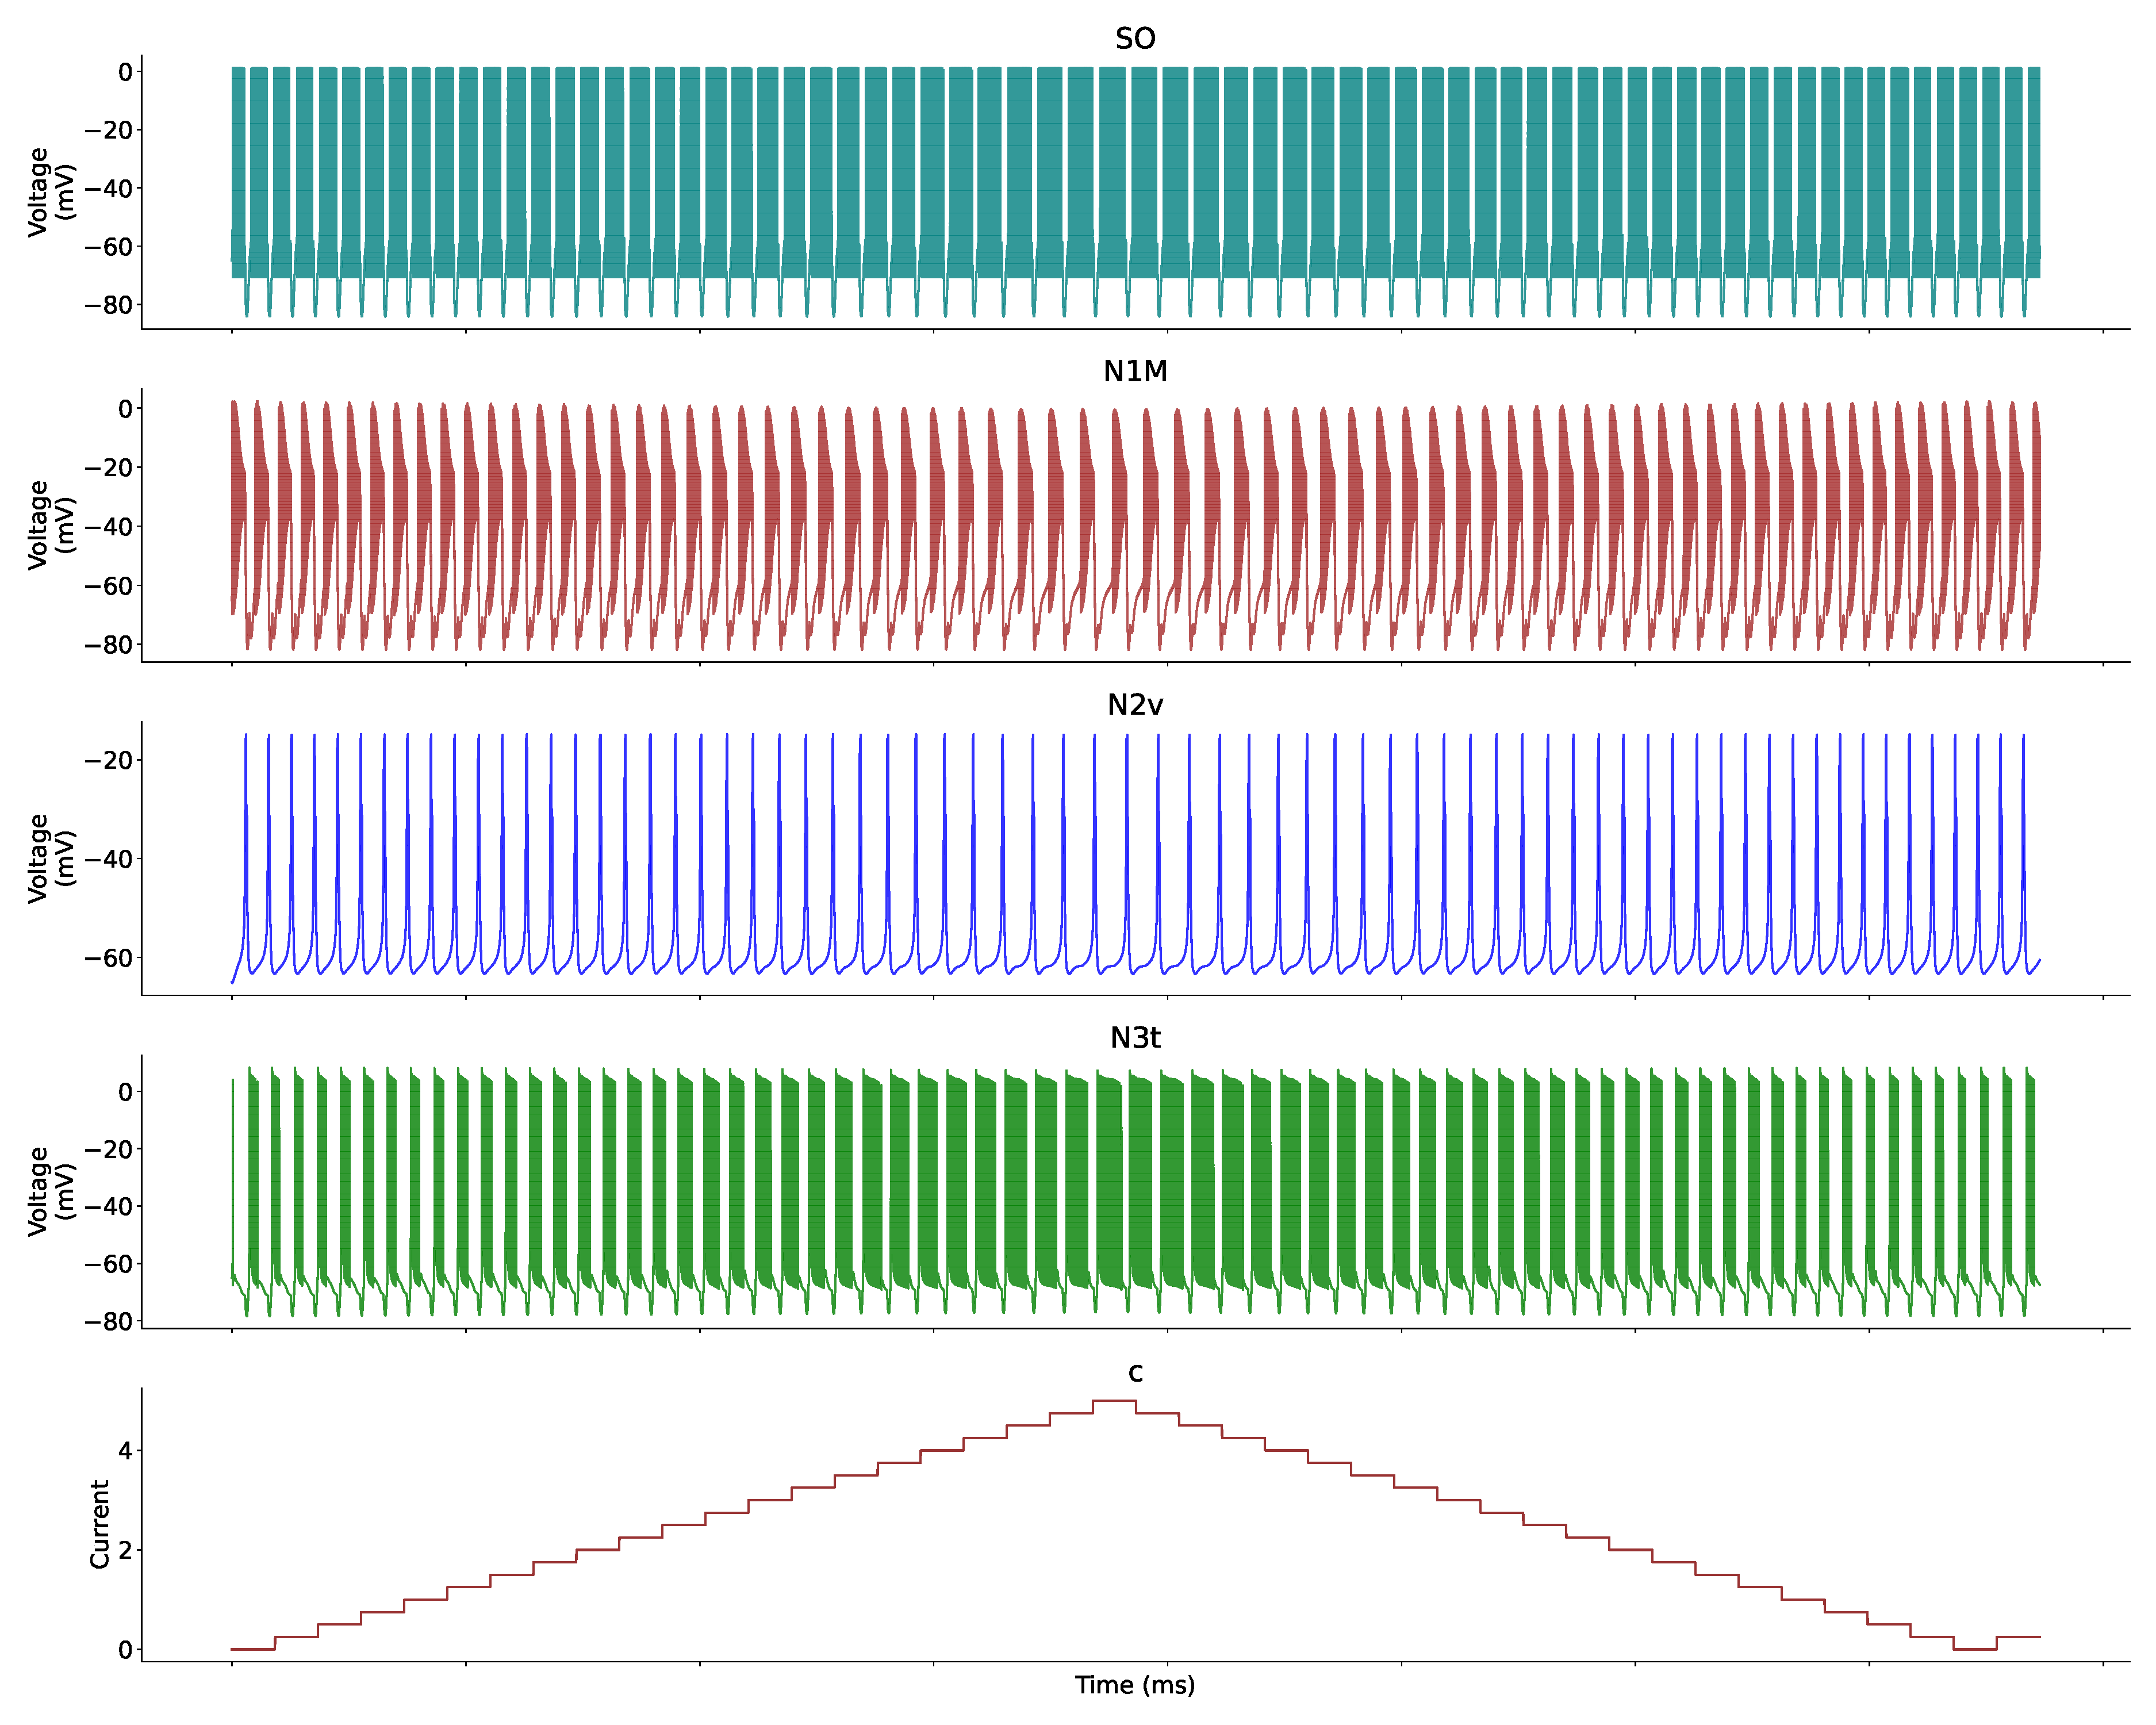
\includegraphics[width=\textwidth]{img/methods-paper-modelo/circuit_w_current.pdf}
	\caption{Illustration of the CPG activity when a current ramp \(i_{inj}\) is applied to N3t. Variability in the sequence intervals was induced by applying two consecutive ramps as the one shown in this figure into different cells. The ramp current was applied only to one of the cells at a time.}
	\label{fig:complete ramp example}
\end{figure}

Whilst the single neuron model descriptions have no intrinsic variability, the effect produced by the modulation of the injected current in each neuron induces variability into the circuit, which allows characterizing the sequence intervals and the period, the associated robustness of the rhythm and the presence of dynamical invariants. Such stimulation has been used previously in the living circuit, as reported by \textcite{elliott_temporal_1991}. The authors of this work showed that it is possible to activate the feeding CPG with variability caused by current injection into individual cells in the circuit. CPG rhythms obtained under this type of stimulation differ depending on which neuron is being stimulated. To induce variability in the model we used a ramp protocol resulting in circuit time-interval variations as in Fig. \ref{fig:complete ramp example}.

% Even though this CPG model do not present intrinsic variability, thanks to the current \(i_{inj}\), variability is induced into the model, effectively changing burst duration. This current injection has also been used in Lymnaea preparation in living elements, stimulating N1M and SO, obtaining rhythm. Neural sequences obtained after the stimulation differ one another depending on which neuron is being stimulated. 


By varying the current injected into N1M, its burst duration is kept nearly constant, but its depolarization phase before the spiking activity begins becomes longer. Since N3t is the neuron fitting in the sequence in that phase (see Fig. \ref{fig:model simulation}), it also increases its burst duration, being the most variable one in the CPG rhythm. 

When value \(i_{inj}\) is increased on neuron SO, its burst duration becomes longer. Since SO has a modulator effect over N3t and N1M, it also alters the burst duration of these two neurons.

Neuron N3t also shows variable burst duration when an evolving current is injected. When \(i_{inj}\) value on N3t is larger, its burst duration increases, elongating the N1M depolarization phase.  

Finally, when current is applied to N2v the effect on its burst duration or the burst duration of the rest of the neurons is rather small. However, \(i_{inj}\) % current 
modulates N2v burst frequency through the hyperpolarization phase. 

%cambios
Therefore, we used a current ramp protocol to induce variability in the CPG model defined as follows: a ramp variable $c$, which controlled the current injection value ($i_{inj}=c$) on the neuron being stimulated, was increased from a minimum to a maximum value, and then decreased back to the initial value. This was repeated twice in each simulation. The ramp variable was modified with a fixed step value every 4.6 seconds (the approximate duration of two N3t bursts). The minimum and maximum $c$ values were different in each cell and were tuned to generate realistic spiking-bursting behavior. All parameters used for the simulation analyses reported in this section are summarized in Table \ref{table:inj values}.

\begin{table}[h!]
\centering
\begin{tabular}{c|cccc|c|ccc|}
\multirow{2}{*}{\textbf{\begin{tabular}[c]{@{}c@{}}Neuron\\ stimulated\end{tabular}}} & \multicolumn{4}{c|}{\textbf{\(i_{inj}\) value}}                 & \multirow{6}{*}{} & \multicolumn{3}{c|}{\textbf{Ramp values ($c$)}}   \\ \cline{2-5} \cline{7-9} 
                                                                                      & \textbf{SO} & \textbf{N1M} & \textbf{N2v} & \textbf{N3t} &                   & \textbf{Min} & \textbf{Max} & \textbf{Step} \\ \cline{1-5} \cline{7-9} 
\textbf{N1M}                                                                          & 8.5         & $c$            & 2            & 0            &                   & 0            & 10.5         & 0.5           \\ \cline{1-5} \cline{7-9} 
\textbf{N3t}                                                                          & 9           & 10           & 1            & $c$            &                   & 0            & 5            & 0.25          \\ \cline{1-5} \cline{7-9} 
\textbf{SO}                                                                           & $c$           & 10           & 1            & 4            &                   & 8.2          & 13           & 0.25          \\ \cline{1-5} \cline{7-9} 
\end{tabular}
\caption{List of \(i_{inj}\) values that yield realistic bursting rhythms for each neuron in the model CPG used in the stimulation protocols reported in this chapter. The left section of the table displays the \(i_{inj}\) values applied to each neuron (columns) during each simulation condition (rows). Ramp values on the right section refer to the minimum and maximum values of the ramp variable $c$ in each simulation, increasing \(i_{inj}\) in the specified step every 4.6 seconds (the approximate duration of two N3t burst) to induce variability.} \label{table:inj values}
\end{table}

Simulations of \textcite{vavoulis_dynamic_2007} model were implemented in C++. The code of the feeding CPG model implementation is available at \href{github.com/GNB-UAM/CPG-feeding-Lymnaea}{https://github.com/GNB-UAM/CPG-feeding-Lymnaea}. This model was also included in Neun library in a Github repository \href{github.com/GNB-UAM/Neun}{https://github.com/GNB-UAM/Neun}. Each simulation had the duration of two consecutive cycles of up and down ramps as the one shown in Fig. \ref{fig:complete ramp example} using the parameters described in Table \ref{table:inj values}. The number of bursts in each simulation was approximately 140 (this number slightly depends on the neuron stimulated). Parameter values such as reversal potentials and synaptic conductances were the same ones specified in \textcite{vavoulis_dynamic_2007}.

\subsection{Experimental recordings and stimulation}
\label{subsec:methods experimental intervals}
The experimental recordings analyzed in section \ref{sec:experimental sussex} were performed by Michael Crossley, University of Sussex, and were kindly provided for this work. 

Each recording had at least 5 microelectrodes, which allowed to characterize the rhythm based on combinations of different neuron's activity. There are cases of experiments in that section:
\begin{itemize}
	\item Spontaneous activity: After the isolation of the CNS, the electrodes impaled in the neuron recorded the spontaneous activity in the CPG, with no further stimulation.
	\item Nerve electrical stimulation: For the activation of the rhythm it is possible to stimulate the median lip nerve (MLN). The data analyzed there was stimulated by a 4V stimulus at 1Hz. 
	\item Neuron electrical stimulation: To modulate the CPG rhythm, SO and CV1a neurons where stimulated (in different experiments) by injecting a constant depolarizing current.
\end{itemize}

To define each phase, we used different neurons and bursting references, depending on the ones available on the circuit, following intervals definition in table \ref{table:cpg ref intervals}.

For each recording each phase was characterized as follows:
\begin{itemize}
    \item Spontaneous Activity Example 1 and 3: N1 phase was analyzed from B1 activity (bursting and depolarization); N2 phase was analyzed from B5 hyperpolarization, which has a strong inhibition from N2v; N3 phase was analyzed from the bursting activity of B8, that replicates the N3t duration. 
    \item Spontaneous Activity Example 2: N1 phase was analyzed from B1 activity (bursting and depolarization); N2 phase was analyzed from B1 hyperpolarization, which has a strong inhibition from N2v; N3 phase was analyzed from the bursting activity of B8, that replicates the N3t duration. Since the reference for N2 here coincides with N1 reference, we display here only the intervals corresponding to N1 and N3 phases, since the intervals that correspond to 3 phases, such as N1-N2 delay or N2-N3 delay, either are already represented in the defined intervals or have a duration close to 0 ms.
    \item SO driven by stimulation and spontaneous: N1 phase was analyzed from B1 activity (bursting and depolarization) and N3 phase was analyzed from the bursting activity of B8, that replicates the N3t duration. N2 phase could not be clearly defined.
    \item MLN driven and CV1a driven 1-4: N1 phase was analyzed from N1M activity by a threshold helped by the derivative of the signal; N3 phase was analyzed from the bursting activity of B8 (analogously to the cases above). In CV1a stimulation for cases 1 and 3 N2 phase was also characterized from the inhibition of N1M. 
\end{itemize}

\subsection{Models with chaotic activity}
\label{sec:model variability equations}
As we discussed in the introduction, there are several models that are able to reproduce intrinsic variability in the voltage dynamics without the introduction of stochastic noise. These models produce deterministic chaos which is useful to reproduce observed biological variability. In this subsection, we include the equations of the models used in Sec. \ref{sec:model variability} to represent variable and non-variable voltage activity.
\subsubsection{LP model by \textcite{nowotny_probing_2008} with chaotic activity}

To illustrate the variability displayed by chaotic models, in Sec. \ref{sec:model variability} we used the model by \textcite{nowotny_probing_2008}, which reproduces the activity of LP neuron in the pyloric CPG. The membrane potential of the axon and soma compartments, $V_{\text{axon}}$ and $V_{\text{soma}}$ respectively, are described in this model by the following equations:

\begin{equation}
	\frac{dV_{\text{axon}}}{dt} = \frac{1}{C_a} \left( -I_{\text{Na}} - I_{\text{Kd}} - I_M - I_{\text{leak,a}} + I_{VV} \right)
\end{equation}

\begin{equation}
	\frac{dV_{\text{soma}}}{dt} = \frac{1}{C_s} \left( -I_{\text{Ca}} - I_{\text{KCa}} - I_A - I_h - I_{\text{leak,s}} - I_{VV} \right)
\end{equation}

All ionic currents except for the ones mentioned explicitly below are given by:

\begin{equation}
	I_x = g_x m^p h^q (V - V_x)
\end{equation}

where $g_x$ is the maximal conductance of the current, $V$ is the membrane potential of either the axon compartment ($I_{\text{Na}}$, $I_{\text{Kd}}$, and $I_M$) or the soma compartment (the rest of the ionic currents), and $V_x$ is the ionic reversal potential. The activation and inactivation variables are described by:

\begin{equation}
	\frac{dm}{dt} = \alpha_m (1 - m) - \beta_m m
\end{equation}

\begin{equation}
	\frac{dh}{dt} = \alpha_h (1 - h) - \beta_h h
\end{equation}

for $I_{\text{Na}}$ and $I_{\text{Kd}}$, and

\begin{equation}
	\frac{dm_x}{dt} = \frac{m_{\infty,x}(V) - m_x}{\tau_{m_x}}
\end{equation}

for the rest of the currents indicated by $x$.

The simulations with this model were performed using the code originally published by the authors. The code is freely available at \href{https://modeldb.science/116957}{https://modeldb.science/116957}.

\subsubsection{Non chaotic model by \textcite{ghigliazza_minimal_2004b}}
The Ghigliazza and Holmes model \parencite{ghigliazza_minimal_2004b} for motoneurons is described by the following equations:

\textbf{1. Membrane Potential Equation}
\begin{equation}
C \frac{dv}{dt} = -[I_{\text{Ca}} + I_{\text{K}} + I_{\text{L}} + I_{\text{KS}}] + I_{\text{ext}}
\end{equation}

\textbf{2. Ionic Currents}
\begin{equation}
I_{\text{Ca}} = \bar{g}_{\text{Ca}} m_{\infty}(v) (v - E_{\text{Ca}})
\end{equation}

\begin{equation}
I_{\text{K}} = \bar{g}_{\text{K}} n (v - E_{\text{K}})
\end{equation}

\begin{equation}
I_{\text{L}} = \bar{g}_{\text{L}} (v - E_{\text{L}})
\end{equation}

\begin{equation}
I_{\text{KS}} = \bar{g}_{\text{KS}} c (v - E_{\text{K}})
\end{equation}

\textbf{3. Gating Variables Dynamics}
\begin{equation}
\frac{dm}{dt} = \frac{\epsilon}{\tau_m(v)} [m_{\infty}(v) - m]
\end{equation}

\begin{equation}
\frac{dc}{dt} = \frac{\delta}{\tau_c(v)} [c_{\infty}(v) - c]
\end{equation}

\textbf{4. Steady-State Activation and Time Constants}
\begin{equation}
w_{\infty}(v; k_{i0}, v_{\text{th}}) = \frac{1}{1 + e^{-k_{i0} (v - v_{\text{th}})}}
\end{equation}

\begin{equation}
\tau_i(v; k_{i0}, v_{\text{th}}) = \text{sech}(k_{i0}(v - v_{\text{th}}))
\end{equation}

\subsection{Hybrot structure}
\label{sec:robot setup}
The experimental paradigm designed in order to test the correct behavior and locomotion of the FLC-Hybrot --FLC stands for Functional Living Circuit \parencite{soetard_dynamical_2023}-- established a real-time closed-loop interaction between the robot and a living pyloric CPG of \textit{Carcinus maenas} \parencite{elices_robust_2019}. During the experiment, the FLC-Hybrot had to walk through a straight and flat lane, with no obstacles, along which there were interspersed sections with lights and shadows. Neural activity was recorded online from the living circuit and used to modulate the robot movement. At the same time, feedback current was injected into the living circuit when the robot's light-sensor detected a shadow.

Top panel of Figure \ref{fig:robot_results_setup} shows an illustration of the experimental setup for the FLC-Hybrot implementation. In the real-time configuration, a computer was the link between the robot and the living preparation (Fig. \ref{fig:robot_results_setup}A). The processes taking part during the real-time protocol were:
\begin{enumerate}
	\item First, reading the online signals received from the amplifiers through the DAQ device (Fig. \ref{fig:robot_results_setup}B), which were recorded from CPG neurons in the living preparation (Figure \ref{fig:robot_results_setup}C).
	\item Extracting from the signal, in real-time, the duration of the temporal intervals of the cycle-by-cycle CPG activity and sending them to the robot's controller via Bluetooth.
	\item In the communication from the robot to the computer, the robot's light-sensor data was sent through the same Bluetooth connection.
	\item When the data indicated that the robot was located under a shadow a signal was sent back to the DAQ. At that moment, a current was injected into the neurons altering their behavior.
\end{enumerate}

All these operations were repeated while the robot traversed the trial track (Figure \ref{fig:robot_results_setup}D). Robot's locomotion was determined by its legs oscillation, so we utilized video tracking tools to capture their movement during the experiment (Figure \ref{fig:robot_results_setup}E). Two electrodes were used in order to measure the pyloric CPG activity. First, an extracellular electrode picked up all the surrounding neurons' activity. In this signal, the spikes and bursts of the LP neuron were clearly recognizable due to their larger amplitude. One of the PD neurons' membrane potential was recorded using an intracellular electrode. A second intracellular electrode was used to inject the feedback current into a PD neuron to implement the robotic sensory feedback (Figure \ref{fig:robot_results_setup}F).

\begin{figure}[h!]
	\begin{center}
		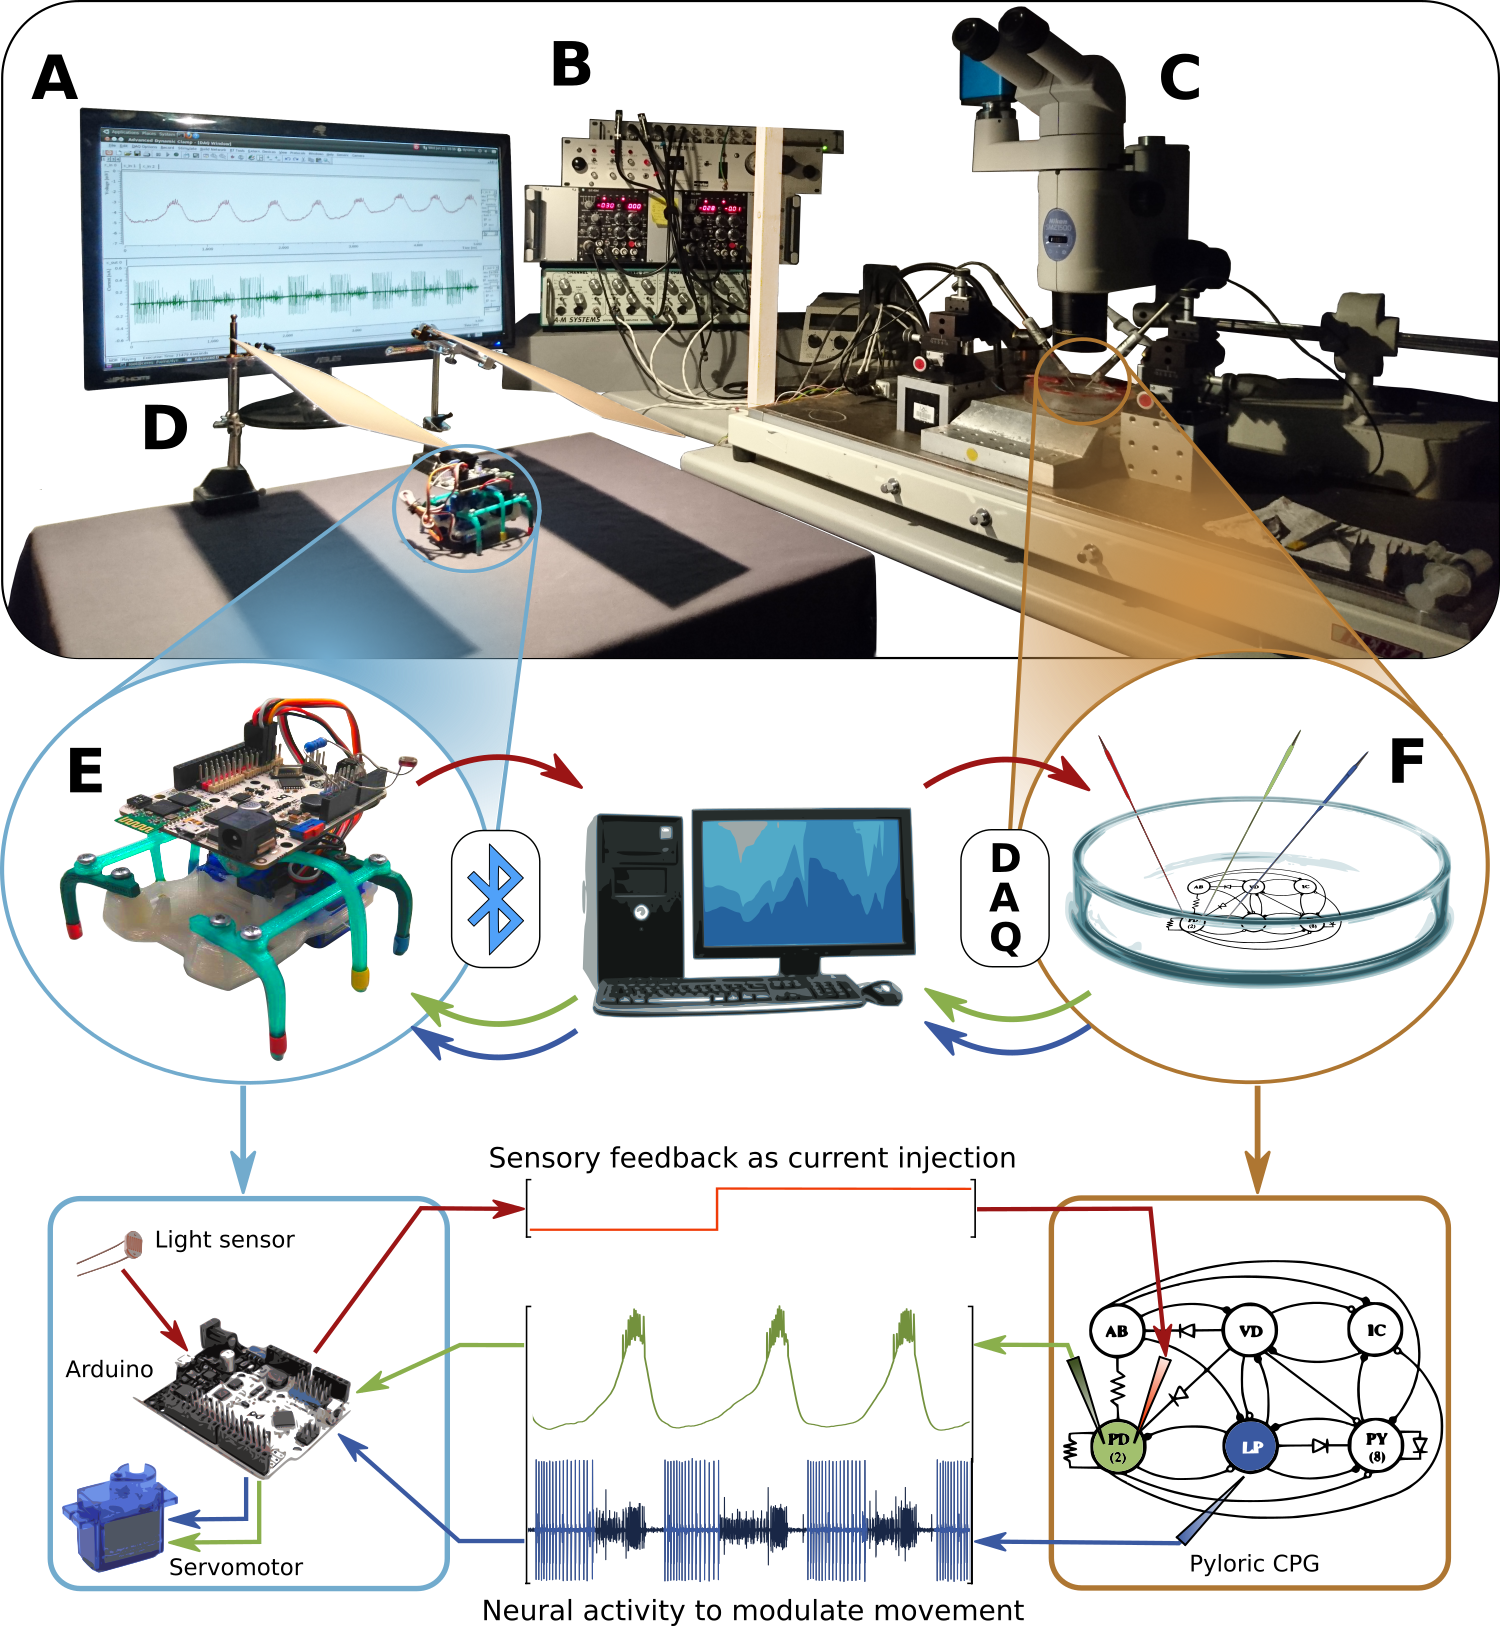
\includegraphics[width=0.65\linewidth]{img/invariants/robot/robot_results_setup.png}
	\end{center}
	\caption{Hybrot experiment design \textbf{Top panel:} illustration of the experimental setup for the FLC-Hybrot implementation: A) Computer controlling the closed-loop interaction between the living CPG and the robot. B) DAQ and signal amplifiers; C) Microscope; D) Testing track with light and shadow regions. \textbf{Middle panel:} Detail of the elements of the setup: E) Hexapod robot, receives the neural information from the computer and sends back the sensory feedback through a Bluetooth connection; F) \textit{In vitro} pyloric CPG preparation with three electrodes to: (1) record extracellular activity from the nerve which includes the activity from the LP neuron (blue) (2) to record intracellular activity from the PD neuron (green) and (3) to introduce the feedback current into a PD neuron (red). The signal recorded from the electrode is received through the DAQ device. \textbf{Bottom panel:} detail of the elements of the robot and the preparation. PD neuron (intracellular recording, green trace) and LP neuron (extracted from the extracellular recording, blue trace) the activity is analyzed online by the computer and used to modulate the movement of the robot. Meanwhile, robot's light sensor detects the presence of light or shadow over it and the Arduino board sends that information to the computer, which injects feedback current into the PD neuron (red trace) accordingly.}
	\label{fig:robot_results_setup}
\end{figure}



\newpage
\clearpage



